\documentclass[tikz]{standalone}

\usepackage{fp}
\usepackage{tikz}
\usepackage{tikz-3dplot}
\usepackage{amsmath} %математические формулы
\usepackage[e]{esvect}  %Красивая стрелочка вектора


\usetikzlibrary{calc}
\usetikzlibrary{arrows.meta}

\input{../tikzcom.tex}

\begin{document}
	
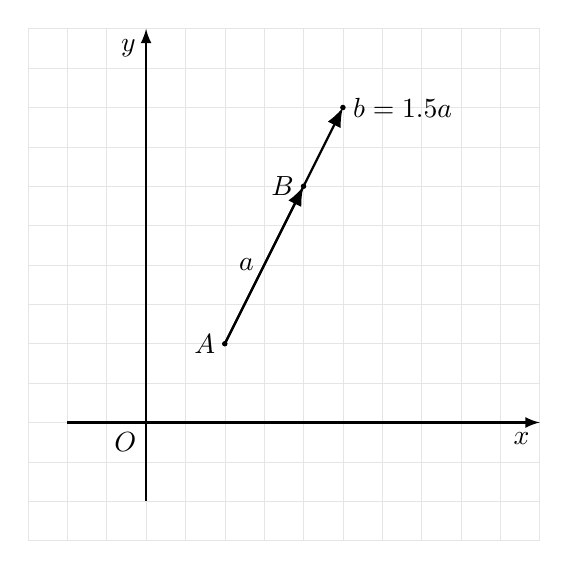
\begin{tikzpicture}[scale=1]
	
	
	\draw[step=.5cm,black!10,very thin] (-1.5,-1.5) grid (5,5);
	
	\draw[-latex, thick] (-1,0) -- (5,0) node [below left] {$x$};
	\draw[-latex, thick] (0,-1) -- (0,5) node [below left] {$y$};
	
	\coordinate (O) at (0,0);
	
	\draw (O) node [below left] {$O$};
	
	
	\coordinate (A) at (1,1);
	\coordinate (B) at (2,3);
	
	
	\fill [black] (A) circle [radius=1pt];
	\fill [black] (B) circle [radius=1pt];
	\fill [black] ($(A)!1.5!(B)$) circle [radius=1pt];
	
	\draw[-{Latex[length=7pt]}, thick] (A) -- (B) node [left, midway] {$\vv{a}$};
	
	\draw[-{Latex[length=7pt]}, thick] (A) -- ($(A)!1.5!(B)$) node [right] {$\vv{b} = 1.5\vv{a}$};
	
	\draw (A) node[left,] {$A$};
	\draw (B) node[left] {$B$};   			
	
	
	
	
\end{tikzpicture}
	
\end{document}